\documentclass[10pt, xcolor={dvipsnames}]{beamer}
\usetheme{Boadilla}
\beamertemplatenavigationsymbolsempty
\setbeamerfont{title}{series=\bfseries}
\setbeamerfont{author}{series=\normalfont}
\setbeamerfont{frametitle}{series=\bfseries}
\setbeamerfont{footline}{series=\bfseries}
\setbeamertemplate{caption}[numbered]
%\setbeamertemplate{page number in head/foot}{}
\usepackage{caption}

\definecolor{links}{HTML}{2A1B81}
\hypersetup{colorlinks,linkcolor=,urlcolor=links}
\setbeamercolor{bibliography item}{fg=black}
\setbeamercolor{bibliography entry author}{fg=black}
\setbeamercolor{bibliography entry title}{fg=black}
\setbeamercolor{bibliography entry location}{fg=black}
\setbeamercolor{bibliography entry note}{fg=black}

\DeclareMathOperator*{\argmin}{arg\,min}
\DeclareMathOperator{\Ex}{\mathbb{E}}
\DeclareMathOperator{\Prob}{\mathbb{P}}
\DeclareMathOperator{\dotp}{{ \bullet }}
\newcommand{\norm}[1]{\left\lVert#1\right\rVert}
\newcommand{\vect}[1]{\boldsymbol{#1}}

\usepackage[utf8x]{inputenc}
\usepackage[english]{babel}

\usepackage{graphicx}
%----------------------------------------------------------------------------------------
%	TITLE PAGE
%----------------------------------------------------------------------------------------

\setbeamerfont{title}{size=\large}
\setbeamerfont{author}{size=\normalsize}
\setbeamerfont{date}{size=\footnotesize}

\title[Max-Cut and Goemans-Williamson]{Max-Cut and Goemans-Williamson}
\author[\textcolor{white}{Marko Lalovic}]{\textcolor{black}{Marko Lalovic} \vspace{-.2cm}}
\date[\textcolor{white}{Aug 2, 2022}]{\textcolor{black}{Summer 2022}}

\defbeamertemplate*{title page}{customized}[1][]
{
  \usebeamerfont{title}\inserttitle\par
  \usebeamerfont{subtitle}\usebeamercolor[fg]{subtitle}\insertsubtitle\par
  \bigskip
  \usebeamerfont{author}\insertauthor\par
  \usebeamerfont{institute}\insertinstitute\par
%  \usebeamerfont{date}\insertdate\par
  \usebeamercolor[fg]{titlegraphic}\inserttitlegraphic
  \bigskip
}

\begin{document}
\begin{frame}
\begin{center}
\maketitle
\begin{figure}
    \includegraphics[width=.8\linewidth]{../figures/front-figure.pdf}
\end{figure}
\end{center}
\end{frame}

\begin{frame}{Outline}
    \tableofcontents
\end{frame}

%----------------------------------------------------------------------------------------
%	SLIDES
%----------------------------------------------------------------------------------------
\section{Max-Cut}
\begin{frame}{Max-Cut}
\begin{itemize}
\item Goal: Given $G = (V, E)$ with $V := \lbrace 1, \dots, n \rbrace$ and $|E| = m$
\item Find a subset $S \subseteq V$, such that $f(S) := |{\color{red}cut(S)}|$ is maximum
\end{itemize}

\begin{center}
\begin{figure}
\includegraphics[width=.3\textwidth]{../figures/max-cut-crop.pdf}
\end{figure}
\end{center}
Max-Cut problem is NP-complete~[Karp72]~\footnote{Karp(1972) Reducibility among Combinatorial Problems}. 
How well can we approximate Max-Cut?
\end{frame}

\begin{frame}{Approximation Algorithms}
\begin{itemize}
\item Denote the optimal value of the Max-Cut problem by $mc(G)$
\item And the size of the cut returned by some algorithm by $alg(G)$
\end{itemize}
\begin{definition}
Algorithm $f(S) = alg(G)$ is an $\alpha$-{\it approximation} of Max-Cut if
\begin{equation}
f(S) \geq \alpha \cdot mc(G)
\label{ineq: definition}
\end{equation}
for all graphs $G = (V, E)$ and some approximation ratio $\alpha \in [0, 1]$.
\end{definition}
If algorithm employed is randomized, we say the same, if Inequality~(\ref{ineq: definition}) holds with an expectation taken on the left-hand side.
\end{frame}

\begin{frame}{Approximation Algorithms}
\begin{example}
Randomized $\frac{1}{2}-$approximation algorithm for Max-Cut, that assigns each vertex of $V$ to $S$ and $V \setminus S$ independently uniformly at random
\begin{equation}
\Ex[f(S)] = \sum_{(i, j) \in E} \Prob[(i, j) \in \text{cut}(S)] = \frac{1}{2} \cdot m \geq \frac{1}{2} \cdot mc(w)
\end{equation}
[Erd67]~\footnote{Erdős(1967) On bipartite subgraphs of a graph}
\end{example}
\begin{itemize}
\item Can we do better?
\item Yes: In preliminary version in `94 of [GW95]~\footnote{Goemans and Williamson(1995) Improved approximation algorithms for maximum cut and
satisfiability problems using semidefinite programming} they improved this by proposing $\alpha_{GW}$-approximation algorithm with $\alpha_{GW} \geq 0.87$ using semidefinite programming.
\end{itemize}
\end{frame}

\section{Preliminaries}
\begin{frame}{Preliminaries}
A real symmetric matrix $X$ is positive definite, denoted $X \succeq 0$ if the following equivalent conditions hold:
\begin{enumerate}
\item All eigenvalues of $X$ are non-negative
\item Quadratic form $v^{T}Xv \geq 0$ for all $v \in \mathbb{R}^{n}$
\item There exists $Q \in \mathbb{R}^{n \times r}$ with 
$$
X = QQ^{T} = \sum_{i = 1}^{r} v_{i} v_{i}^{T}
$$
where $v_{1}, \dots, v_{r}$ are columns of $Q$
\end{enumerate}
\end{frame}

\begin{frame}{Preliminaries}
\begin{itemize}
\item Let $S^{n}_{+}$ denote the convex cone of positive semidefinite matrices in the set of all symmetric matrices $S^{n}$ 
\item A {\it \color{red} spectrahedron} is the intersection of $S^{n}_{+}$ with an affine linear space $L$
\end{itemize}
\vspace{0.5cm}
\begin{center}
\begin{figure}
\includegraphics[width=.44\textwidth]{../figures/cone-crop.pdf}
\end{figure}
\end{center}
\end{frame}

\begin{frame}{Semidefinite Programming}
\begin{itemize}
\item {\it Semidefinite programming (SDP)} solves the following problem: maximize or minimize a linear objective function over the spectrahedron:
\end{itemize}
\begin{align}
& \text{maximize} \ C \dotp X \nonumber\\
& \text{subject to: } \label{eq: P} \tag{P}\\
& \qquad A_{i} \dotp X  = b_{i} \quad i = 1, \dots, m \nonumber\\
& \qquad X \succeq 0 \nonumber\\
\nonumber\\
& \text{minimize} \ b^{T}y \nonumber\\
& \text{subject to: } \label{eq: P} \tag{D}\\
& \qquad \sum_{i=1}^{m} A_{i} y_{i} - C \succeq 0 \nonumber
\end{align}

\begin{itemize}
\item {\it Weak duality}: $C \dotp X \geq b^{T} y$ always holds 
\item Under primal and dual feasibility, also {\it strong duality}: $C \dotp X = b^{T} y$ holds
\end{itemize}

\end{frame}

\section{SDP Relaxation}

\begin{frame}{Reformulation of Max-Cut}
\begin{itemize}
\item The optimal value of the Max-Cut problem can be expressed by
\begin{equation}
mc(G) =\max_{x \in \lbrace -1, 1 \rbrace^{n}} \sum_{i, j} \frac{1 - x_{i} x_{j}}{2}
\tag{{\color{red} QP}}
\end{equation}
\end{itemize}
\begin{example}[$K_{3}$]
\begin{minipage}[t]{0.3\textwidth}
\vspace{1cm}
\begin{figure}
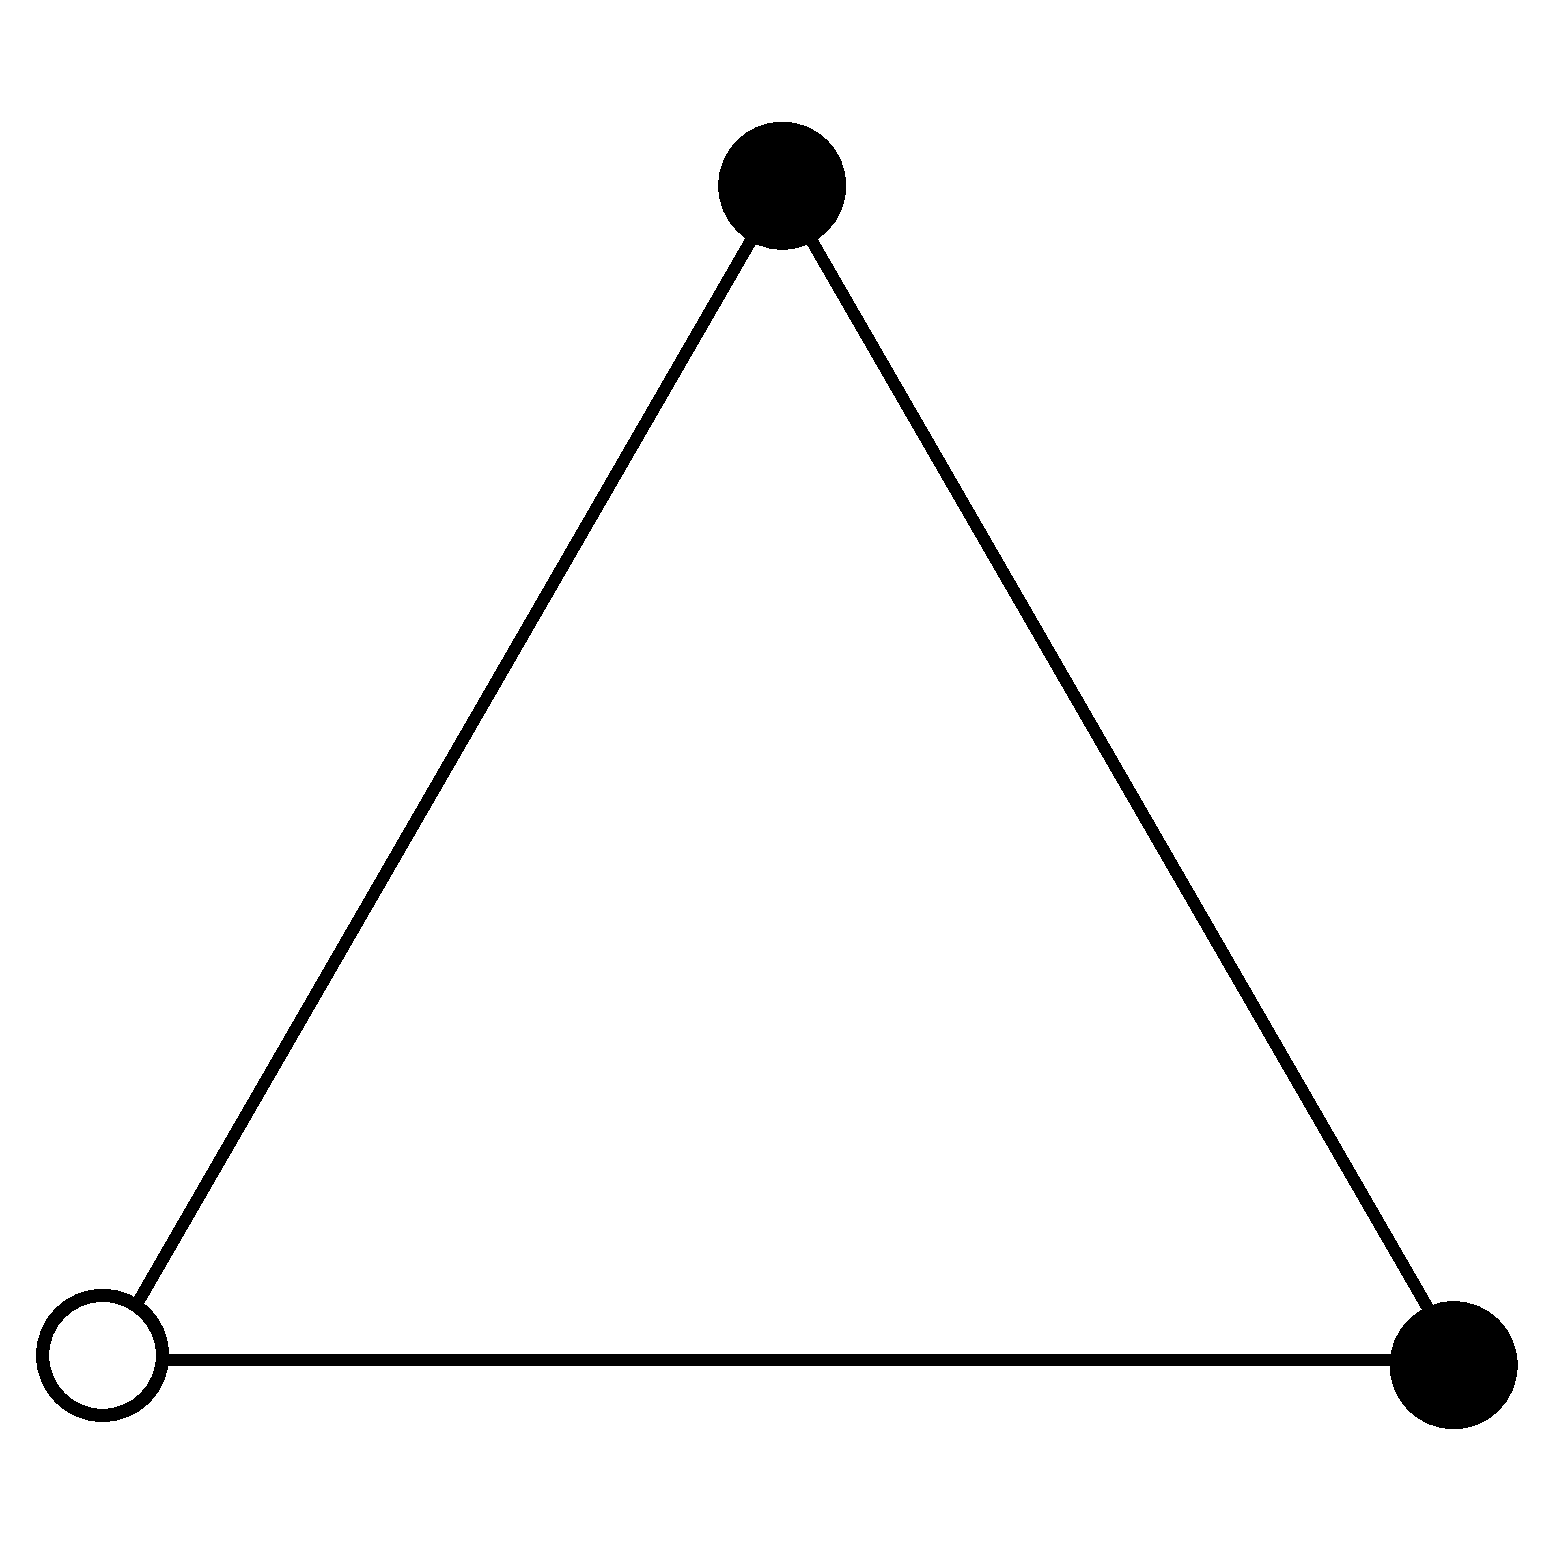
\includegraphics[width=.5\textwidth]{../figures/k3.pdf}
\end{figure}
\end{minipage}%%%%%%%%%%%%%%%%
\begin{minipage}[t]{0.5\textwidth}
\vspace{2mm}
\begin{align*}
&\text{If: } \quad
(x_1, x_2, x_3)^{T} = (1, -1, -1)^{T} \\
&\text{Then: }
\end{align*}
\begin{align*}
mc(G) &= \frac{1 - x_1 x_2}{2} + 
\frac{1 - x_1 x_3}{2} +
\frac{1 - x_2 x_3}{2} \\
&= 
\frac{1 - 1 (-1)}{2} + 
\frac{1 - 1 (-1)}{2} +
\frac{1 - (-1) (-1)}{2} \\
&= 1 + 1 + 0\\
&= 2
\end{align*}
\end{minipage}
\end{example}
\end{frame}

\begin{frame}{SDP Relaxation Cont.}
\begin{itemize}
\item Cuts in the complete graph $K_n$ can be represented by
$$\lbrace x x^{T} : x \in \lbrace -1, 1 \rbrace^{n} \rbrace$$ 
\item The {\it elliptope} $\mathcal{E}_{n}$ is a set of all $n \times n$ correlation matrices 
\begin{equation}
\mathcal{E}_{n} = \lbrace X \in S_{n} : X_{ii} = 1 \quad \text{for all $i$} \rbrace
\end{equation}
\end{itemize}

\begin{example}[$K_{3}$]
\begin{minipage}[t]{0.5\textwidth}
\begin{figure}
\includegraphics[width=.8\textwidth]{../figures/Elliptope.pdf}
\end{figure}
\end{minipage}
\begin{minipage}[t]{0.5\textwidth}
\vspace{2mm}
$$
\begin{pmatrix}
1 & x & y\\
x & 1 & z\\
y & z & 1
\end{pmatrix} \succeq 0
\text{ and } x,y,z \in [-1, 1]
$$
\begin{align*}
&\text{If: } \quad
(x, y, z)^{T} = (1, -1, -1)^{T} \\
&\text{Then: }
\end{align*}
\vspace{-1cm}
$$
X = \begin{pmatrix}
1 & -1 & -1\\
1 & 1 & -1\\
-1 & -1 & 1
\end{pmatrix}
$$
\end{minipage}
\end{example}
\end{frame}

\begin{frame}{SDP Relaxation}
\begin{itemize}
\item Therefore
\begin{align}
mc(G) &=
\max_{X \in \mathcal{E}_{n}, rk(X) = 1 } \sum_{i, j} \frac{1 - X_{ij}}{2}\nonumber\\ 
&\leq
\max_{X \in \mathcal{E}_{n}} \sum_{i, j} \frac{1 - X_{ij}}{2} = sdp(G)
\label{eq: relaxation}
\end{align}
\item This means that $sdp(G)$ is a {\it relaxation} of Max-Cut problem.
\item {\color{red}Note}: Objective function is linear in entries of matrix $X$
\end{itemize}
\end{frame}

\section{Hyperplane Rounding}
\begin{frame}{Hyperplane Rounding}
Every positive semidefinite matrix $X$ can be decomposed as $X = QQ^{T}$ and the quantity $sdp(G)$ can be reformulated as
\begin{equation}
sdp(G) = \max_{\norm{v_{i}}_{2} = 1} \sum_{i, j} \frac{1 - v_{i}^{T} v_{j}}{2}
\end{equation}

Select a random unit vector $r \in \mathbb{R}^{n}$ and construct the subset 
$$
S := \lbrace i \in V \mid v_{i}^{T}r \geq 0 \rbrace
$$
This is called {\it hyperplane rounding}
\end{frame}

\begin{frame}{Hyperplane Rounding}
We can show that
\begin{equation}
\Ex[f(S)] = \sum_{i, j} \Prob[(i, j) \in cut(S)] \geq \alpha_{GW} \cdot sdp(G)
\label{eq: lower-bound}
\end{equation}
where $\alpha_{GW} = \min_{\theta_{i, j} \in [0, \pi]} \lbrace 
\frac{2}{\pi}\frac{\theta_{i, j}}{ { 1 - \cos(\theta_{i, j}) }} \rbrace \geq 0.878$. 
Combining Inequalities~\ref{eq: relaxation} and~\ref{eq: lower-bound}
\begin{equation}
\Ex[f(S)] \geq \alpha_{GW} \cdot sdp(G) \geq \alpha_{GW} \cdot mc(G)
\end{equation}
and finally conclude
\begin{equation}
\Ex[f(S)] \geq \alpha_{GW} \cdot mc(G)
\end{equation}
\end{frame}

\begin{frame}{Sketch of Proof of (7)}
\begin{equation}
\Prob[(i, j) \in cut(S)] = \frac{\theta_{i, j}}{\pi}
\end{equation}

\begin{center}
\begin{figure}
\includegraphics[width=.5\textwidth]{../figures/hyperplane-rounding-crop.pdf}
\end{figure}
\end{center}
\end{frame}

\begin{frame}{Sketch of Proof of (7) Cont.}
\begin{align*}
\Prob[(i, j) \in cut(S)] &= \frac{\theta_{i, j}}{\pi} \\
&=\frac{\arccos(v_{i}^{T}v_{j})}{\pi}\\
&=\frac{\color{red}2}{\pi}\frac{\arccos(v_{i}^{T}v_{j})}{ {\color{red} 1 - v_{i}^{T}v_{j} }}  \frac{\color{red}1 - v_{i}^{T} v_{j} }{\color{red}2} \\
&\geq \min_{\theta_{i, j} \in [0, \pi]} \lbrace 
\frac{2}{\pi}\frac{\theta_{i, j}}{ { 1 - \cos(\theta_{i, j}) }} 
\rbrace \cdot
\frac{1 - v_{i}^{T} v_{j} }{2}\\
&= \alpha_{GW} \cdot \frac{1 - v_{i}^{T} v_{j} }{2}\\
&= \alpha_{GW} \cdot sdp(G)
\end{align*}
\end{frame}

\section{Dual Problem}
\begin{frame}{Dual Problem}
\begin{itemize}
\item Warm up: find maximum eigenvalue of a symmetric matrix $X \in S^{n}_{+}$
\item Suppose $X$ has eigenvalues
\begin{equation}
\lambda_{1} \geq \dots \geq \lambda_{n}
\end{equation}
\item Then for some $t \in \mathbb{R}$
\begin{equation}
t - \lambda_{1} \leq \dots \leq t - \lambda_{n}
\end{equation}
\item Note: $t I - X \succeq 0$ if and only if $0 \leq t - \lambda_{1}$ or equivalently $t \geq \lambda_{\max}(X)$
\item This immediately gives us an SDP
\begin{equation}
\lambda_{\max}(X) = \min_{t}\lbrace t I - X \succeq 0 \rbrace   
\end{equation}
\end{itemize}
\end{frame}

\begin{frame}{Dual Problem}
Define the {\it Laplacian matrix} $L = (L_{i,j})_{i,j}$ of a graph $G = (V, E)$ as
\begin{equation}
L_{i,j} := \begin{cases}
deg(v_i)   &\text{if $i = j$}\\
-1  &\text{if $(i, j) \in E(G)$}\\
0   &\text{otherwise}
\end{cases}
\end{equation}
Dual of Max-Cut SDP relaxed problem can be reformulated as
\begin{align}
& \text{minimize} \ \frac{n}{4} t \nonumber\\
& \text{subject to: } \tag{D'}\\
& \qquad t I - (L + diag(u)) \succeq 0 \nonumber\\
& \qquad \vect{1}^{T}u = 0 \nonumber
\end{align}
\end{frame}

\begin{frame}{Dual Problem}
Dual of Max-Cut SDP relaxed problem can be reformulated as:
\begin{equation}
\frac{n}{4} \min_{u: \vect{1}^{T} u = 0} \lambda_{\max}(L + diag(u))
\end{equation}

By weak duality we get an upper bound given in [MP90]~\footnote{Mohar and Poljak(1990) Eigenvalues and the max-cut problem}
\begin{equation}
mc(G) \leq sdp(G) \leq \frac{n}{4} \lambda_{\max}(L)
\end{equation}

For $G = C_5$, $\lambda_{\max} = \frac{1}{5}(5 + \sqrt{5})$, we get the upper bound studied in [DP93]~\footnote{Delorme and Poljak(1993) Laplacian eigenvalues
and the maximum cut problem}
\begin{equation}
\frac{1}{2}(5 + \sqrt{5})/4 \geq 0.9 \cdot mc(C_{n})
\end{equation}
\end{frame}

\section{SoS Relaxation}
\begin{frame}{SoS Relaxation}
Find an operator $\tilde{\Ex}$ that behaves like the expectation over some probability distribution on $x \in \lbrace 0, 1 \rbrace^{n}$
\begin{equation}
\tilde{\Ex}: \mathcal{P}^{\leq d}_{n} \rightarrow \mathbb{R}
\end{equation}
where ${P}^{\leq d}_{n}$ represents a set of polynomials $p: \lbrace 0, 1 \rbrace^{n} \rightarrow \mathbb{R}$ of degree at most $d$ in $n$ variables $x_1, \dots x_n$, {\color{red} $x_{i} \in \lbrace 0, 1 \rbrace$}, to get an optimization problem for Max-Cut:
\begin{align}
& \text{max}_{\tilde{\Ex}} \ \tilde{\Ex}[ \sum_{(i, j) \in E(G)} (x_{i} - x_{j})^{2} ] \nonumber\\
& \text{subject to: } \label{eq: P} \tag{D''}\\[.4em]
& \qquad \text{(1) $\tilde{\Ex}$ is linear} \qquad \text{(2) $\tilde{\Ex}[1] = 1$} \nonumber\\[.4em]
& \qquad \text{(3) $\tilde{\Ex}[p^2] \geq 0$} \qquad \, \, \, \text{\color{red} (4) $\tilde{\Ex}[x_{i}^{2}p] = \tilde{\Ex}[x_{i}p]$} \nonumber\\[.4em]
& \qquad \text{for all polynomials $p$ with $deg(p) \leq \frac{d}{2}$}\nonumber
\end{align}
\end{frame}

\begin{frame}{SoS Relaxation}
\begin{itemize}
\item This is a relaxation of Max-Cut problem
\item  Given $G= (V, E)$ and a subset $S$ with size of the cut $mc(G)$, there is a feasible solution to (D'') with objective value equal to $mc(G)$
\begin{itemize}
\item Denote the indicator vector of $S$ as $a_1, \dots, a_n$ and let $\tilde{\Ex}$ be
\begin{equation}
\tilde{\Ex}[p(x_1, \dots, x_n)] = p(a_1, \dots, a_n)
\end{equation}
\item Then $\tilde{\Ex}$ satisfies the constraints (1)-(4) and achieves objective value 
\begin{equation}
\tilde{\Ex}[ \sum_{(i, j) \in E(G)} (x_{i} - x_{j})^{2} ] = mc(G)
\end{equation}
\end{itemize}
\item This approach is called {\it Sum-of-Squares (SoS)} hierarchy and was introduced in [Pa00]~\footnote{Parrilo(2000) Structured semidefinite programs and semi-algebraic geometry methods in robustness and optimization} and~[La01]~\footnote{Lasserre(2001) Global optimization with polynomials
and the problem of moments}
\item Increasing the degree $d$, we increase the size of SDP problem. For $d = n$, we get exact relaxation
\end{itemize}
\end{frame}

\section{Gaussian Rounding}
\begin{frame}{Gaussian Rounding}
Given $\tilde{\Ex}$ that realizes the maximum in (D''), i.e.\ SDP solution of SoS with objective value
\begin{equation}
sos(G) := \text{max}_{\tilde{\Ex}} \ \tilde{\Ex}[ \sum_{(i, j) \in E(G)} (x_{i} - x_{j})^{2} ]
\end{equation}
From SoS being a relaxation of Max-Cut it also follows that
\begin{equation}
sos(G) \geq mc(G) \qquad \text{for all $G = (V, E)$}
\label{eq: upper-bound-sos}
\end{equation}
\end{frame}

\begin{frame}{Gaussian Rounding}
\begin{itemize}
\item Assume $\tilde{\Ex}[x_i] = \frac{1}{2}$ for all $i = 1, \dots n$
\item Take $y$ to be a Gaussian vector with the following mean and covariance matrix
\begin{equation}
\mu = \tilde{\Ex}[x] = \frac{1}{2} \vect{1} \qquad \Sigma = \tilde{\Ex}[(x - \mu)(x - \mu)^{T}]
\end{equation}
\item Construct the indicator vector $a$ for a subset $S \subseteq V$ as
\begin{equation}
a_i = \begin{cases}
1,  &\text{if $y_{i} \leq \frac{1}{2}$}\\
0,  &\text{otherwise}
\end{cases}
\end{equation}
\end{itemize}
\end{frame}

\begin{frame}{Gaussian Rounding}
We can show that
\begin{equation}
\Ex[f(S)] = \sum_{i, j}  \Prob[(i, j) \in cut(S)] \geq \alpha_{GW} \cdot 
sos(G)
\label{eq: lower-bound-sos}
\end{equation}
where $\alpha_{GW} = \min_{\theta \in [0, \pi]} \lbrace \frac{2}{\pi}\frac{\theta}{1 - \cos(\theta)} \rbrace \geq 0.878$ as before. Combining Inequalities \ref{eq: upper-bound-sos} and~\ref{eq: lower-bound-sos}
$$
\Ex[f(S)] \geq \alpha_{GW} \cdot sos(G) \geq \alpha_{GW} \cdot mc(G)
$$
we can also in this case conclude that
\begin{equation}
\Ex[f(S)] \geq \alpha_{GW} \cdot mc(G)
\end{equation}
\end{frame}

\begin{frame}{Sketch of Proof of (25)}
\begin{itemize}
\item For each edge $(i, j) \in E(G)$, define $\rho_{i, j} = 4 \tilde{\Ex}[x_{i} x_{j}] - 1$
\item Given two uncorrelated random variables $(s, t) \overset{\text{i.i.d.}}{\sim} N(0, I)$, we can get $\rho_{i, j}$-correlated random variables $s$ and $u$, where
\begin{equation}
u = \rho_{i, j} s + \sqrt{1 - \rho_{i, j}^{2}} t
\end{equation}
\item Then $\rho_{i, j} = \Ex[u s] = \cos(\theta_{i, j})$, and we can calculate
\begin{align*}
\Prob[(i, j) \in cut(S)] 
&= \Prob[a_i \neq a_j]\\
&= \Prob[sgn(y_i - \frac{1}{2}) \neq sgn(y_{j} - \frac{1}{2})] \\
&= \Prob[sgn(s) \neq sgn(u)] \\
&= \frac{\theta_{i, j}}{\pi}
\end{align*}
\end{itemize}
\end{frame}

\begin{frame}{Sketch of Proof of (25) Cont.}
\vspace{-.4cm}
\begin{align*}
\Ex[f(S)] &= \sum_{i, j}  \Prob[(i, j) \in cut(S)] \\
&= \sum_{i, j} \frac{\theta_{i, j}}{\pi} \\
&= \sum_{i, j} \frac{\theta_{i, j}}{\pi} \cdot {\color{red} \frac{2}{(1 - \rho_{i, j})} \tilde{\Ex}[(x_{i} - x_{j})^{2}]} \\
&= \sum_{i, j} \frac{2}{\pi} \frac{\theta_{i, j}}{1 - \cos(\theta_{i, j})} 
\tilde{\Ex}[(x_{i} - x_{j})^{2}] \\
&\geq \min_{\theta \in [0, \pi]} \lbrace 
\frac{2}{\pi}\frac{\theta}{ { 1 - \cos(\theta) }} 
\rbrace \cdot 
\sum_{i, j}\tilde{\Ex}[(x_{i} - x_{j})^{2}]\\
&= \alpha_{GW} \cdot \sum_{i, j}\tilde{\Ex}[(x_{i} - x_{j})^{2}]\\
&= \alpha_{GW} \cdot \tilde{\Ex}[\sum_{i, j}(x_{i} - x_{j})^{2}]\\
&= \alpha_{GW} \cdot sos(G)
\end{align*}
\end{frame}

\end{document}